
In this section we'll go over several commands that can be very useful for automating certain bits of code.

\subsection{Grouped Command Execution}
One of the easiest ways we can repeat a certain command for different groups of observations is with the \st{bysort} prefix.
This prefix lets us run the command we use it with for every group defined by a variable separately.
In my experience it's mostly useful for generating variables in programming,
but it can also be used as a quick and dirty way to compare variables across groups.
We can use the prefix like so: \st{bysort varlist: command},
where \st{varlist} is a list of the variables -- or a single variable --identifying the different groups,
and \st{command} is the command we would like to run.
Note that \st{bysort varlist:} is equivalent to using \st{by varlist, sort:}.
The \st{by} prefix does not work without sorting the data, so it is generally easier to just use \st{bysort}.
\cref{lst:sort} provides an example.

\begin{listing}[tbp]
\caption{bysort.do}\label{lst:sort}
\inputst{bysort.do}
\end{listing}

\subsection{Conditionals}
Conditionals, or if-statements, are where the real fun stuff begins.
To put it simply,
they allow us to differentiate our code based on anything we can turn into an expression that evaluates to true or false.
Stata recognises two types of if-statements: one as a command suffix,
and one for programming.
In this section,
we'll first go over expressions before we move on to the two types of if-statements.

\subsubsection{Expressions}
When we use conditionals,
we set requirements that must hold for code to be executed.
An expression can then be seen as a check whether these requirements are fulfilled.
An expression always evaluates to true or false:
the requirements are met, or they are not.
In programming, we refer to a data type that has either the value ``true'' or ``false'' as a \emph{boolean}.
An evaluated expression is precisely that.
In programming,
true and false are often represented by $1$ and $0$, respectively.
This is also the case in Stata:
if we look at dummy variables,
for example,
they function in much the same way.
A dummy variable for gender is often coded in such a way that it represents either male or female,
such as a variable \st{female} with value $1$ for females and value $0$ for males.

Expressions are much like mathematical equations,
in that they have a left-hand side,
a relational operator,
and a right-hand side.
Based on the relational operator,
the left-hand side is compared to the right-hand side,
and the expression is evaluated to be true or false.
Let's take a look at an example.
Suppose we have two scalars, $a$ and $b$,
and want to check whether these are equal to one another.
First, we need to have these scalars defined.
Let's say that $a=3$ and $b=\pi$:
\begin{minted}{stata}
// define scalars
sca a = 3
sca b = c(pi)

// inspect the values of the scalars
di "Scalar a holds value " a
di "Scalar b holds value " b
\end{minted}
We then want Stata to tell us whether $a=b$:
\begin{minted}[firstnumber=9]{stata}
// show whether a and b are equal
di a == b
\end{minted}
Of course, clever as we are, we know this to be false.
This expression should therefore evaluate to false, i.e., $0$.
When we run this code, we see that, indeed, the last command returns $0$ (see \cref{fig:exp}).

\begin{figure}[tbp]\centering
    \caption{Stata output for expression code}\label{fig:exp}
    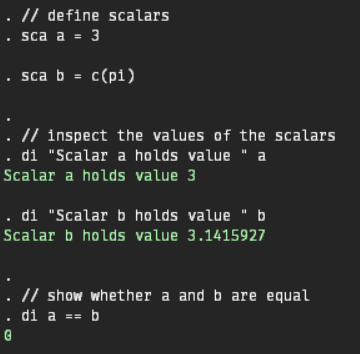
\includegraphics[width=0.5\textwidth]{expression.png}
\end{figure}

Of course, we don't always want to know whether things are equal to one another.
Luckily, there are more relational operators than just \st{==} (equals).
To see the full list of available operators,
type \st{help operator} in the command window.
Furthermore, we may want to set more than one requirement.
Luckily, we can combine multiple requirements using logic operators -- also listed in \st{help operator}.

Suppose we now want to know whether $a \leq b$.
We could then tell Stata to tell us whether $a = b$ \emph{or} $b > a$ is true:\footnote{%
Of course, this can also be achieved using a single $\leq$ operator,
but for the sake of the example I don't do that here.}
\begin{minted}[firstnumber=12]{stata}
// show whether a and b are equal, or b is larger than a
di a == b | b > a
\end{minted}
As $\pi > 3$, this will evaluate to true.
Try for yourself using the code in \cref{lst:expression}!

\begin{listing}[tbp]
\caption{expression.do}\label{lst:expression}
\inputst{expression.do}
\end{listing}


\subsubsection{Command suffix if}
The command suffix if statement is the simpler of the two.
By adding an if-statement to the end of a command (but before the options!) we tell Stata to only use the specified subset of our data.
You've likely done this before,
but let's go over an example.
First, we'll use one of Stata's example datasets:
\begin{minted}{stata}
// load example dataset
sysuse auto, clear

// inspect available variables
describe
\end{minted}

Here, the variable \st{foreign} is a dummy variable indicating whether the origin of a car is foreign (value $1$), or domestic (value $0$).
Suppose now we want some descriptive statistics,
but only for imported cars.
We do this by adding an if-statement to the \st{summarize} command that evaluates to true only for foreign cars.
Before we do this,
recall the way Stata handles true/false data:
using the values $1$ and $0$.
When ``splitting'' our data based on a dummy variable,
we can exploit this to write very compact if-statements,
like so:
\begin{minted}[firstnumber=7]{stata}
// summary statistics of foreign cars
sum if foreign
\end{minted}
As the dummy already indicates whether it is true that the car is foreign (by taking a value of $1$),
we no longer have to add a relational operator.
Of course, we could do so, but it would be redundant;
we would effectively telling Stata \emph{do }x \emph{if it is true that }y \emph{is true}.
For illustrative purposes,
the code to do so here would be \st{sum if foreign == 1}.

Note that we can use this same ``trick'' when generating our own dummy variables.
Suppose we want to create a dummy indicating whether a car in the dataset is expensive,
say, has a price equal to or over 10,000\$.\footnote{%
I'm just going to assume the prices in this dataset are in dollars,
as the currency isn't really mentioned in the dataset.}
The way I used to do this is as follows:
\begin{minted}{stata}
// generate dummy for expensive cars
gen expensive = 1 if price >= 10000
replace rexpensive = 0 if price < 10000
\end{minted}
But we could actually just write
\begin{minted}[firstnumber=10]{stata}
// generate dummy for expensive cars
gen expensive = price >= 10000
\end{minted}
to get exactly the same variable!
See for yourself using \cref{lst:suffix}.

\begin{listing}[tbp]
\caption{suffix-if.do}\label{lst:suffix}
\inputst{suffix-if.do}
\end{listing}

\subsubsection{Programming if}
Stata's programming if-statements have a multitude of uses.
They allow us to execute bits of code only if a specified expression is true.
We'll continue with a similar example as in \cref{lst:expression};
but now we want Stata to tell us whether scalar \st{a} is larger than scalar \st{b}.
Let's begin with defining the scalars.
Instead of picking the values ourselves,
we'll have Stata pick a number for us, ranging from 1--10:\footnote{%
I use the function \st{runiformint()} for this,
so that Stata only returns whole numbers, or integers.
If we want Stata to pick \emph{any} real number instead,
we could instead use the function \st{runiform()}.}
\begin{minted}{stata}
// define scalars
sca a = runiformint(0, 10)
sca b = runiformint(0, 10)
\end{minted}
We'll also tell Stata to show us the value of both scalars,
so that we can make sure the expression is evaluated correctly:
\begin{minted}[firstnumber=5]{stata}
// display the value of a
di as text "Scalar a holds value " as result a
di as text "Scalar b holds value " as result b
\end{minted}
Finally, we'll add an if-statement:
\begin{minted}[firstnumber=9]{stata}
// display which scalar is larger
if      a > b   di as text "The largest scalar is " as result "a"
\end{minted}

The if-statement can be broken down in three parts.
First, we tell Stata we want to run some code conditonally,
so we start our command with \st{if}.
After writing \st{if}, we add the expression to be evaluated,
which in this case is \st{a > b}.
Finally, we end with the command we want Stata to execute if the expression evaluates to true.
In the example,
this is a display command telling the user that scalar \st{a} is the larger of the two scalars.
Note that with our current code,
if the expression is evaluated to be false,
Stata will do nothing.
To change this,
we can add another line starting with \st{else},
that tells Stata what to do instead.
Furthermore,
we can follow up this \st{else} with another \st{if} to check for other conditions:
\begin{minted}[firstnumber=11]{stata}
else if a < b   di as text "The largest scalar is " as result "b"
else            di as text "Both scalars are equal"
\end{minted}
In a case like this, when we're exhausting all possible options,
the final \st{else} does not need an \st{if}:
if the first two expressions are false,
then the final possibility, i.e. \st{a == b}, must necessarily be true,
so we can leave the conditional out.
Try changing the values of the scalars yourself to see what happens using \cref{lst:if}.

\begin{listing}[tbp]
\caption{programming-if.do}\label{lst:if}
\inputst{programming-if.do}
\end{listing}

We can also execute multiple commands following an if-statement.
To do this, we use code blocks.
Code blocks are multiple lines of code that ``belong together'',
and we use curly brackets to denote the start and end of a code block.
Note that nothing -- other than comments -- can follow an opening curly bracket,
and the closing curly bracket must be on its own line --
other than comments after it.
Furthermore,
the code in a code block is generally indented to make it clear what belongs together,
although this is not necessary.
As an example,
suppose we again want to compare scalars \st{a} and \st{b},
but now only want to know the value of the largest one.
Instead of using \cref{lst:if},
we could instead use the code in \cref{lst:ifblock}.

\begin{listing}[tbp]
\caption{programming-if-block.do}\label{lst:ifblock}
\inputst{programming-if-block.do}
\end{listing}

\subsection{Loops}

Loops are a way to have Stata repeat certain code for a given number of times,
or \emph{over} a given amount of \emph{items}.
Combined with conditionals,
loops allow us to automate tasks that could take a lot of work to write out by hand.
Stata has three different kinds of loops;
\st{forvalues}, \st{foreach}, and \st{while},
and we'll go over each in this subsection.
All three of these make use of locals,
so if you need a refresher on these,
see \cref{sec:macros}.

\subsubsection{Looping over values}

Looping over values is the most straightforward type of loop.
It allows us to repeat a piece of code a predefined amount of times,
while keeping track of the current iteration in a local.
The command for this type of loop is \st{forvalues}.
Suppose we want to have Stata show the numbers 1--10.
We can then run a loop repeating the \st{display} command ten times:
\begin{minted}{stata}
// repeat display command ten times
forvalues i = 1/10 {
    // display current value of local
    di as text "Current value: " as result "`i'"
}
\end{minted}
Note that the structure of a loop is similar to that of an if-statement:
we first declare the loop using \st{forvalues},
we then have an expression defining over what values we're looping,
and we finish with a code block containing the code to be repeated.

Before moving on to some more complex examples,
I'd like to elaborate a bit on the middle part, the expression.
The syntax of this expression is always \texttt{\textit{localname} = \textit{range}},
so that we both define the name of the local to keep track of the iterations,
as well as the range of values (and thus amount of iterations) that the loop covers.
Make sure that you do not use a localname that is already being used in your current program,
as the loop would then overwrite the contents of the existing local.
There are four of ways to define the \texttt{\textit{range}} of values.
I'd like to highlight two of these here.
The first of the two, \st{a/b}, is used in the previous example,
and counts from \st{a} to \st{b} in steps of one.\footnote{%
Note that this is in steps of \emph{positive} one: a range defined like this only counts ``up''.}
I'll illustrate the second with another example.
Suppose we would like to use display only the \emph{odd} number in 1--10.
To do this, we could construct an if-statement that only displays the current iteration if it is odd,
or we could ``count'' in steps of two:
\begin{minted}[firstnumber=7]{stata}
// using only odd numbers
forvalues i = 1(2)10 {
    // display current value of local
    di as text "Current value: " as result "`i'"
}
\end{minted}
In this case, we use \st{a(b)c} to define our range:
we count from \st{a} to \st{c}, in steps of \st{b}.
This also allows us to count down: to do so,
we choose our values in such a way that $a>c, b<0$.

While looping over a range of numbers might not seem that useful in and of itself,
if you get creative there is a lot you can do with just this.
To illustrate, I'll provide a more complex example using almost everything we've learned thus far.
Before running the code,
see if you can figure out how it works on your own!
\begin{minted}[firstnumber=13]{stata}
/* a more complex example */
// load example dataset
sysuse auto, clear

// sort by make of car
sort make

// obtain the average price using summary statistics
sum price
sca avg_price   = r(mean)

// display some information on the first ten cars
// loop over values 1 to 10
forvalues i = 1/10 {

    // is it a foreign or domestic car?
    if foreign[`i'] loc car_origin  = "an imported car"
    else            loc car_origin  = "a domestic car"

    // is the price above or below average?
    if price[`i'] > avg_price   loc car_price   = "above average"
    else                        loc car_price   = "below average"

    // display the information
    di as result make[`i'] as text " is " as result "`car_origin'" as text ", and its price is " as result "`car_price'" as text "."
}
\end{minted}

There is one new ``trick'' I'm using in this code:
by adding an index to a variable name, I obtain its value for a specific observation,
like so: \st{varname[index]},
where \textit{\texttt{varname}} is the name of a variable,
and \textit{\texttt{index}} is the index number of an observation.\footnote{%
I might move this to \cref{sec:info} later, as it can be quite a useful trick.}
So what does the code do, exactly?
After loading in the data,
we first sort it alphabetically based on the make of the cars.
We then obtain the average price and store that value in a scalar.
After that, we use a loop to go over the first ten observations.
For each of these, we store in a local whether the care is domestic or foreign,
and whether its price is above or below average.
At the end of the loop,
we display all obtained information, including the make of the car.

\begin{center}\texttt{insert figure with output here}\end{center}

All code used in this specific subsection can be found in \cref{lst:forvalues}.

\begin{listing}[tbp]
\caption{forvalues.do}\label{lst:forvalues}
\inputst{forvalues.do}
\end{listing}

\subsubsection{Looping over items}

\st{foreach}

\subsubsection{Looping until a condition is met}

\st{while}
